% Graphic for TeX using PGF
% Title: D:\INSA\3INFO\PROJETINFO\diagrammes dia\doc_opening.mts
% Creator: Dia v0.97.2
% CreationDate: Wed Apr 22 11:03:23 2015
% For: Utilisateur
% \usepackage{tikz}
% The following commands are not supported in PSTricks at present
% We define them conditionally, so when they are implemented,
% this pgf file will use them.
\ifx\du\undefined
  \newlength{\du}
\fi
\setlength{\du}{15\unitlength}
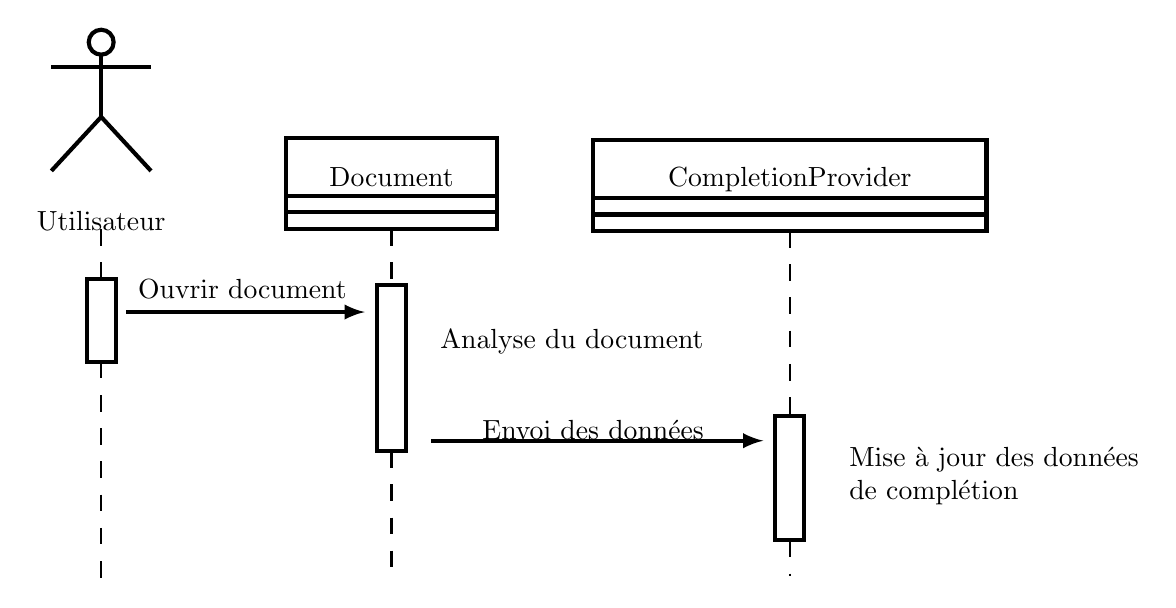
\begin{tikzpicture}
\pgftransformxscale{1.000000}
\pgftransformyscale{-1.000000}
\definecolor{dialinecolor}{rgb}{0.000000, 0.000000, 0.000000}
\pgfsetstrokecolor{dialinecolor}
\definecolor{dialinecolor}{rgb}{1.000000, 1.000000, 1.000000}
\pgfsetfillcolor{dialinecolor}
\pgfsetlinewidth{0.100000\du}
\pgfsetdash{}{0pt}
\definecolor{dialinecolor}{rgb}{1.000000, 1.000000, 1.000000}
\pgfsetfillcolor{dialinecolor}
\pgfpathellipse{\pgfpoint{-28.150000\du}{2.050000\du}}{\pgfpoint{0.300000\du}{0\du}}{\pgfpoint{0\du}{0.300000\du}}
\pgfusepath{fill}
\definecolor{dialinecolor}{rgb}{0.000000, 0.000000, 0.000000}
\pgfsetstrokecolor{dialinecolor}
\pgfpathellipse{\pgfpoint{-28.150000\du}{2.050000\du}}{\pgfpoint{0.300000\du}{0\du}}{\pgfpoint{0\du}{0.300000\du}}
\pgfusepath{stroke}
\definecolor{dialinecolor}{rgb}{0.000000, 0.000000, 0.000000}
\pgfsetstrokecolor{dialinecolor}
\draw (-29.350000\du,2.650000\du)--(-26.950000\du,2.650000\du);
\definecolor{dialinecolor}{rgb}{0.000000, 0.000000, 0.000000}
\pgfsetstrokecolor{dialinecolor}
\draw (-28.150000\du,2.350000\du)--(-28.150000\du,3.850000\du);
\definecolor{dialinecolor}{rgb}{0.000000, 0.000000, 0.000000}
\pgfsetstrokecolor{dialinecolor}
\draw (-28.150000\du,3.850000\du)--(-29.350000\du,5.150000\du);
\definecolor{dialinecolor}{rgb}{0.000000, 0.000000, 0.000000}
\pgfsetstrokecolor{dialinecolor}
\draw (-28.150000\du,3.850000\du)--(-26.950000\du,5.150000\du);
% setfont left to latex
\definecolor{dialinecolor}{rgb}{0.000000, 0.000000, 0.000000}
\pgfsetstrokecolor{dialinecolor}
\node at (-28.150000\du,6.345000\du){Utilisateur};
\pgfsetlinewidth{0.100000\du}
\pgfsetdash{}{0pt}
\definecolor{dialinecolor}{rgb}{1.000000, 1.000000, 1.000000}
\pgfsetfillcolor{dialinecolor}
\fill (-16.300000\du,4.400000\du)--(-16.300000\du,5.800000\du)--(-6.822500\du,5.800000\du)--(-6.822500\du,4.400000\du)--cycle;
\definecolor{dialinecolor}{rgb}{0.000000, 0.000000, 0.000000}
\pgfsetstrokecolor{dialinecolor}
\draw (-16.300000\du,4.400000\du)--(-16.300000\du,5.800000\du)--(-6.822500\du,5.800000\du)--(-6.822500\du,4.400000\du)--cycle;
% setfont left to latex
\definecolor{dialinecolor}{rgb}{0.000000, 0.000000, 0.000000}
\pgfsetstrokecolor{dialinecolor}
\node at (-11.561250\du,5.350000\du){CompletionProvider};
\definecolor{dialinecolor}{rgb}{1.000000, 1.000000, 1.000000}
\pgfsetfillcolor{dialinecolor}
\fill (-16.300000\du,5.800000\du)--(-16.300000\du,6.200000\du)--(-6.822500\du,6.200000\du)--(-6.822500\du,5.800000\du)--cycle;
\definecolor{dialinecolor}{rgb}{0.000000, 0.000000, 0.000000}
\pgfsetstrokecolor{dialinecolor}
\draw (-16.300000\du,5.800000\du)--(-16.300000\du,6.200000\du)--(-6.822500\du,6.200000\du)--(-6.822500\du,5.800000\du)--cycle;
\definecolor{dialinecolor}{rgb}{1.000000, 1.000000, 1.000000}
\pgfsetfillcolor{dialinecolor}
\fill (-16.300000\du,6.200000\du)--(-16.300000\du,6.600000\du)--(-6.822500\du,6.600000\du)--(-6.822500\du,6.200000\du)--cycle;
\definecolor{dialinecolor}{rgb}{0.000000, 0.000000, 0.000000}
\pgfsetstrokecolor{dialinecolor}
\draw (-16.300000\du,6.200000\du)--(-16.300000\du,6.600000\du)--(-6.822500\du,6.600000\du)--(-6.822500\du,6.200000\du)--cycle;
\pgfsetlinewidth{0.050000\du}
\pgfsetdash{}{0pt}
\pgfsetdash{{0.400000\du}{0.400000\du}}{0\du}
\definecolor{dialinecolor}{rgb}{0.000000, 0.000000, 0.000000}
\pgfsetstrokecolor{dialinecolor}
\draw (-28.150000\du,6.550000\du)--(-28.150000\du,7.750000\du);
\definecolor{dialinecolor}{rgb}{0.000000, 0.000000, 0.000000}
\pgfsetstrokecolor{dialinecolor}
\draw (-28.150000\du,9.750000\du)--(-28.150000\du,14.987500\du);
\pgfsetlinewidth{0.100000\du}
\pgfsetdash{}{0pt}
\definecolor{dialinecolor}{rgb}{1.000000, 1.000000, 1.000000}
\pgfsetfillcolor{dialinecolor}
\fill (-28.500000\du,7.750000\du)--(-28.500000\du,9.750000\du)--(-27.800000\du,9.750000\du)--(-27.800000\du,7.750000\du)--cycle;
\definecolor{dialinecolor}{rgb}{0.000000, 0.000000, 0.000000}
\pgfsetstrokecolor{dialinecolor}
\draw (-28.500000\du,7.750000\du)--(-28.500000\du,9.750000\du)--(-27.800000\du,9.750000\du)--(-27.800000\du,7.750000\du)--cycle;
\pgfsetlinewidth{0.100000\du}
\pgfsetdash{}{0pt}
\definecolor{dialinecolor}{rgb}{1.000000, 1.000000, 1.000000}
\pgfsetfillcolor{dialinecolor}
\fill (-23.700000\du,4.350000\du)--(-23.700000\du,5.750000\du)--(-18.612500\du,5.750000\du)--(-18.612500\du,4.350000\du)--cycle;
\definecolor{dialinecolor}{rgb}{0.000000, 0.000000, 0.000000}
\pgfsetstrokecolor{dialinecolor}
\draw (-23.700000\du,4.350000\du)--(-23.700000\du,5.750000\du)--(-18.612500\du,5.750000\du)--(-18.612500\du,4.350000\du)--cycle;
% setfont left to latex
\definecolor{dialinecolor}{rgb}{0.000000, 0.000000, 0.000000}
\pgfsetstrokecolor{dialinecolor}
\node at (-21.156250\du,5.300000\du){Document};
\definecolor{dialinecolor}{rgb}{1.000000, 1.000000, 1.000000}
\pgfsetfillcolor{dialinecolor}
\fill (-23.700000\du,5.750000\du)--(-23.700000\du,6.150000\du)--(-18.612500\du,6.150000\du)--(-18.612500\du,5.750000\du)--cycle;
\definecolor{dialinecolor}{rgb}{0.000000, 0.000000, 0.000000}
\pgfsetstrokecolor{dialinecolor}
\draw (-23.700000\du,5.750000\du)--(-23.700000\du,6.150000\du)--(-18.612500\du,6.150000\du)--(-18.612500\du,5.750000\du)--cycle;
\definecolor{dialinecolor}{rgb}{1.000000, 1.000000, 1.000000}
\pgfsetfillcolor{dialinecolor}
\fill (-23.700000\du,6.150000\du)--(-23.700000\du,6.550000\du)--(-18.612500\du,6.550000\du)--(-18.612500\du,6.150000\du)--cycle;
\definecolor{dialinecolor}{rgb}{0.000000, 0.000000, 0.000000}
\pgfsetstrokecolor{dialinecolor}
\draw (-23.700000\du,6.150000\du)--(-23.700000\du,6.550000\du)--(-18.612500\du,6.550000\du)--(-18.612500\du,6.150000\du)--cycle;
\pgfsetlinewidth{0.050000\du}
\pgfsetdash{}{0pt}
\pgfsetdash{{0.400000\du}{0.400000\du}}{0\du}
\definecolor{dialinecolor}{rgb}{0.000000, 0.000000, 0.000000}
\pgfsetstrokecolor{dialinecolor}
\draw (-21.156250\du,6.550000\du)--(-21.156250\du,7.900000\du);
\definecolor{dialinecolor}{rgb}{0.000000, 0.000000, 0.000000}
\pgfsetstrokecolor{dialinecolor}
\draw (-21.156250\du,11.900000\du)--(-21.156250\du,14.937500\du);
\pgfsetlinewidth{0.100000\du}
\pgfsetdash{}{0pt}
\definecolor{dialinecolor}{rgb}{1.000000, 1.000000, 1.000000}
\pgfsetfillcolor{dialinecolor}
\fill (-21.506250\du,7.900000\du)--(-21.506250\du,11.900000\du)--(-20.806250\du,11.900000\du)--(-20.806250\du,7.900000\du)--cycle;
\definecolor{dialinecolor}{rgb}{0.000000, 0.000000, 0.000000}
\pgfsetstrokecolor{dialinecolor}
\draw (-21.506250\du,7.900000\du)--(-21.506250\du,11.900000\du)--(-20.806250\du,11.900000\du)--(-20.806250\du,7.900000\du)--cycle;
\pgfsetlinewidth{0.050000\du}
\pgfsetdash{}{0pt}
\pgfsetdash{{0.400000\du}{0.400000\du}}{0\du}
\definecolor{dialinecolor}{rgb}{0.000000, 0.000000, 0.000000}
\pgfsetstrokecolor{dialinecolor}
\draw (-11.561250\du,6.600000\du)--(-11.561250\du,11.050000\du);
\definecolor{dialinecolor}{rgb}{0.000000, 0.000000, 0.000000}
\pgfsetstrokecolor{dialinecolor}
\draw (-11.561250\du,14.050000\du)--(-11.561250\du,14.900000\du);
\pgfsetlinewidth{0.100000\du}
\pgfsetdash{}{0pt}
\definecolor{dialinecolor}{rgb}{1.000000, 1.000000, 1.000000}
\pgfsetfillcolor{dialinecolor}
\fill (-11.911250\du,11.050000\du)--(-11.911250\du,14.050000\du)--(-11.211250\du,14.050000\du)--(-11.211250\du,11.050000\du)--cycle;
\definecolor{dialinecolor}{rgb}{0.000000, 0.000000, 0.000000}
\pgfsetstrokecolor{dialinecolor}
\draw (-11.911250\du,11.050000\du)--(-11.911250\du,14.050000\du)--(-11.211250\du,14.050000\du)--(-11.211250\du,11.050000\du)--cycle;
\pgfsetlinewidth{0.100000\du}
\pgfsetbuttcap
\pgfsetdash{}{0pt}
{
\definecolor{dialinecolor}{rgb}{0.000000, 0.000000, 0.000000}
\pgfsetfillcolor{dialinecolor}
% was here!!!
\pgfsetarrowsstart{latex}
\definecolor{dialinecolor}{rgb}{0.000000, 0.000000, 0.000000}
\pgfsetstrokecolor{dialinecolor}
\draw (-21.800000\du,8.550000\du)--(-27.550000\du,8.550000\du);
}
% setfont left to latex
\definecolor{dialinecolor}{rgb}{0.000000, 0.000000, 0.000000}
\pgfsetstrokecolor{dialinecolor}
\node at (-24.750000\du,8.000000\du){Ouvrir document};
% setfont left to latex
\definecolor{dialinecolor}{rgb}{0.000000, 0.000000, 0.000000}
\pgfsetstrokecolor{dialinecolor}
\node[anchor=west] at (-20.250000\du,9.250000\du){Analyse du document};
\pgfsetlinewidth{0.100000\du}
\pgfsetbuttcap
\pgfsetdash{}{0pt}
{
\definecolor{dialinecolor}{rgb}{0.000000, 0.000000, 0.000000}
\pgfsetfillcolor{dialinecolor}
% was here!!!
\pgfsetarrowsstart{latex}
\definecolor{dialinecolor}{rgb}{0.000000, 0.000000, 0.000000}
\pgfsetstrokecolor{dialinecolor}
\draw (-12.200000\du,11.650000\du)--(-20.200000\du,11.650000\du);
}
% setfont left to latex
\definecolor{dialinecolor}{rgb}{0.000000, 0.000000, 0.000000}
\pgfsetstrokecolor{dialinecolor}
\node at (-16.300000\du,11.400000\du){Envoi des données};
% setfont left to latex
\definecolor{dialinecolor}{rgb}{0.000000, 0.000000, 0.000000}
\pgfsetstrokecolor{dialinecolor}
\node[anchor=west] at (-10.400000\du,12.100000\du){Mise à jour des données};
% setfont left to latex
\definecolor{dialinecolor}{rgb}{0.000000, 0.000000, 0.000000}
\pgfsetstrokecolor{dialinecolor}
\node[anchor=west] at (-10.400000\du,12.900000\du){de complétion};
\end{tikzpicture}
